%!TEX root=thesis.tex
\chapter{Galaxies and Active Galactic Nuclei}
\label{cha:astro}

    Modern astronomy relies on observations of deep space. Telescopes image the
    sky in different wavelengths, with different wavelengths carrying different
    physical meanings. Infrared surveys detect star formation and dust in
    distant galaxies, and radio surveys detect massive objects called active
    galactic nuclei. In this section, I introduce the physics of what we see
    when we look at the sky in these wavelengths, as well as introducing
    specific radio and infrared surveys relevant to this thesis. I will also
    discuss the motivation behind cross-identifying active galactic nuclei with
    their host galaxies, as well as the inherent difficulty in doing so, and
    hence provide the motivation behind this thesis.

        % \todo{Talk about how black holes are predicted by GR.}

        %     More information on black holes and general relativity can be found in \citet{wald10}.

        % \todo{Talk about how we can observe black holes?}

    \section{Radio Active Galactic Nuclei}
    \label{sec:agns}

        \begin{figure}[!ht]
            \centering
            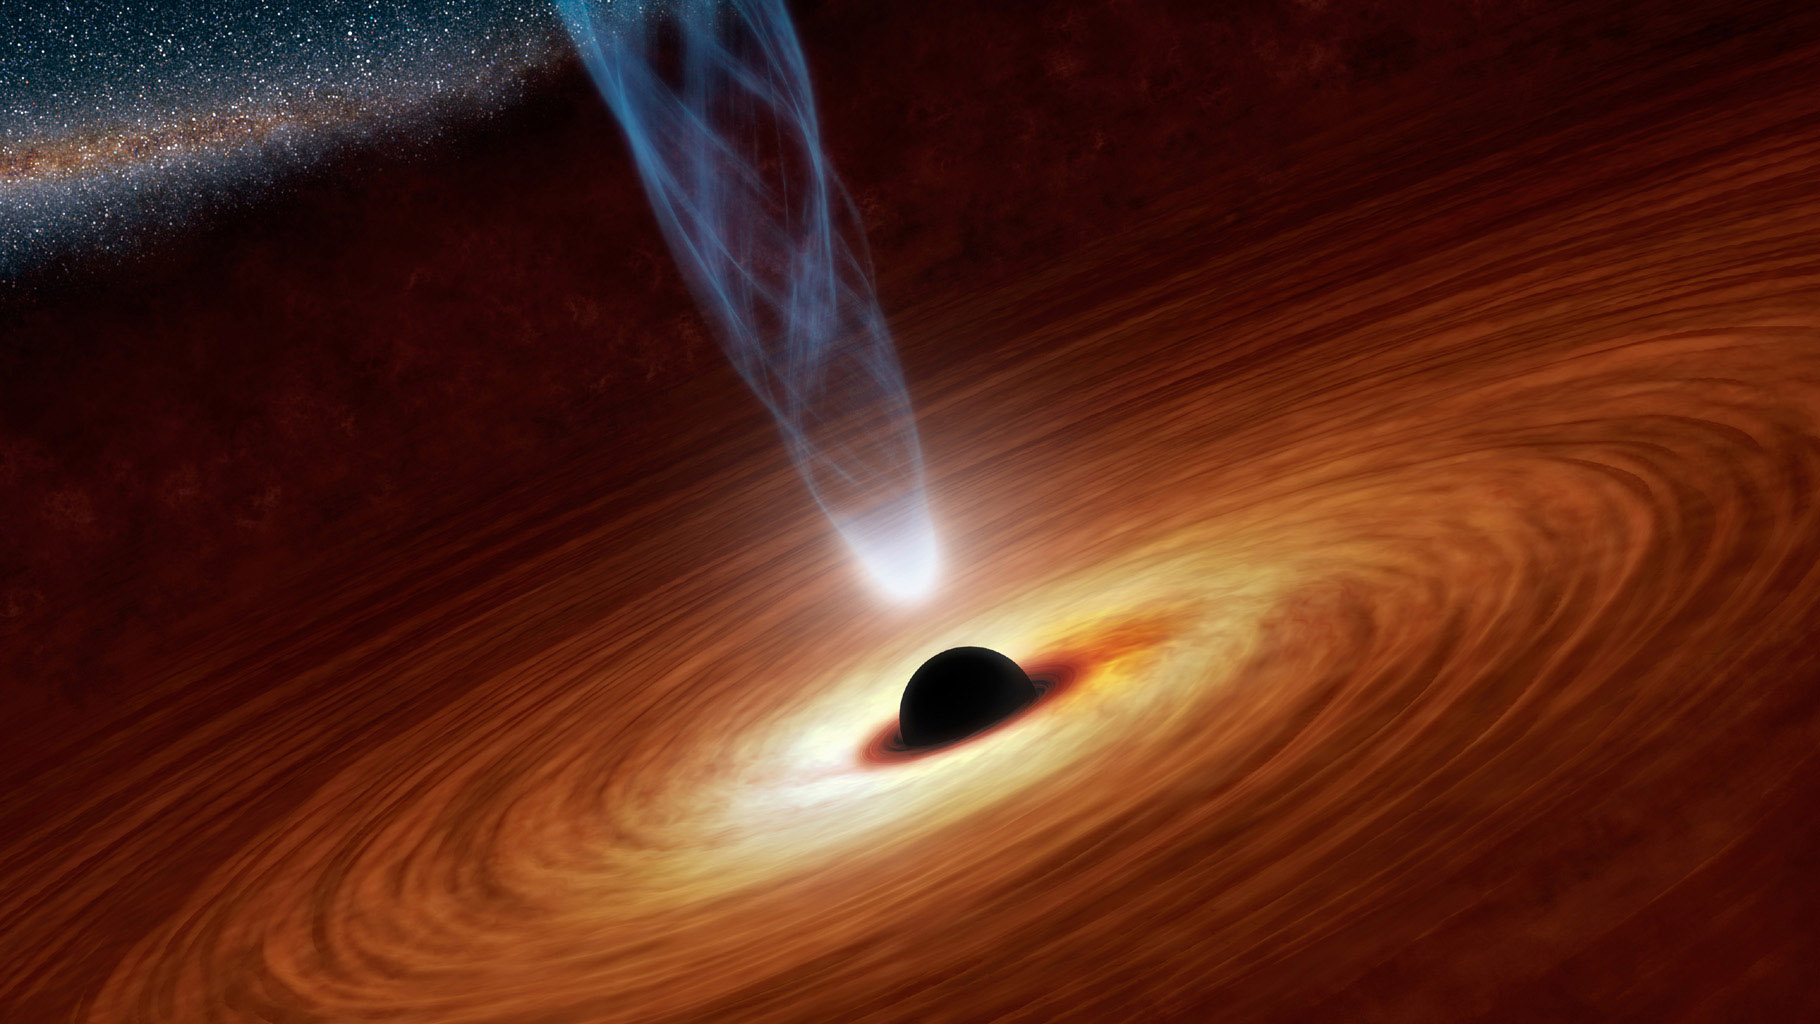
\includegraphics[width=0.8\textwidth]{images/accretion_disk_artist_impression.jpg}
            \caption{An artist's impression of the accretion disk of an active galactic nucleus. \emph{Image: NASA/JPL-Caltech}}
            \label{fig:accretion-disk}
        \end{figure}

        Many galaxies contain a supermassive black hole in their centre. These
        black holes accrete matter from the surrounding galaxy in an
        \emph{accretion disk} (Figure \ref{fig:accretion-disk}). The accretion
        process emits huge amounts of light through different physical
        processes. These light-emitting black holes are called active galactic
        nuclei (AGNs). AGNs can be extremely bright, emitting up to $10^{39}$ J
        of energy every second --- nearly a thousand times more energy than our
        entire galaxy emits \citep{begelman84}. AGNs are found throughout the
        universe: The closest known AGN is Centaurus A (shown in Figure
        \ref{fig:centaurus-a}), with $z \approx 0.0018$, and AGNs have been
        detected up to redshifts of $z \approx 7$ \todo{citation needed}.

        \begin{figure}[!ht]
            \centering
            \includegraphics[width=0.5\textwidth]{images/ESO_Centaurus_A_LABOCA.jpg}
            \caption{Centaurus A, a relatively close radio active galactic
                nucleus. \emph{Image: ESO/WFI (Optical); MPIfR/ESO/APEX/A.Weiss
                et al. (Submillimetre); NASA/CXC/CfA/R.Kraft et al. (X-ray)}}
            \label{fig:centaurus-a}
        \end{figure}

        AGNs produce \emph{jets} from their accretion disk. Jets are long, thin
        streams of matter such as the one shown in Figure \ref{fig:m87}. These
        jets can be very long, with ``giant'' AGNs emitting jets up to 1 Mpc in
        length \todo{citation needed --- maybe \citet{banfield16}?}. The process
        through which jets are emitted is currently unknown \todo{citation
        needed}.        %--- for example, the jet in Figure \ref{fig:m87} is $1.5$ kpc in length \citep{rees87}.

        \begin{figure}[!ht]
            \centering
            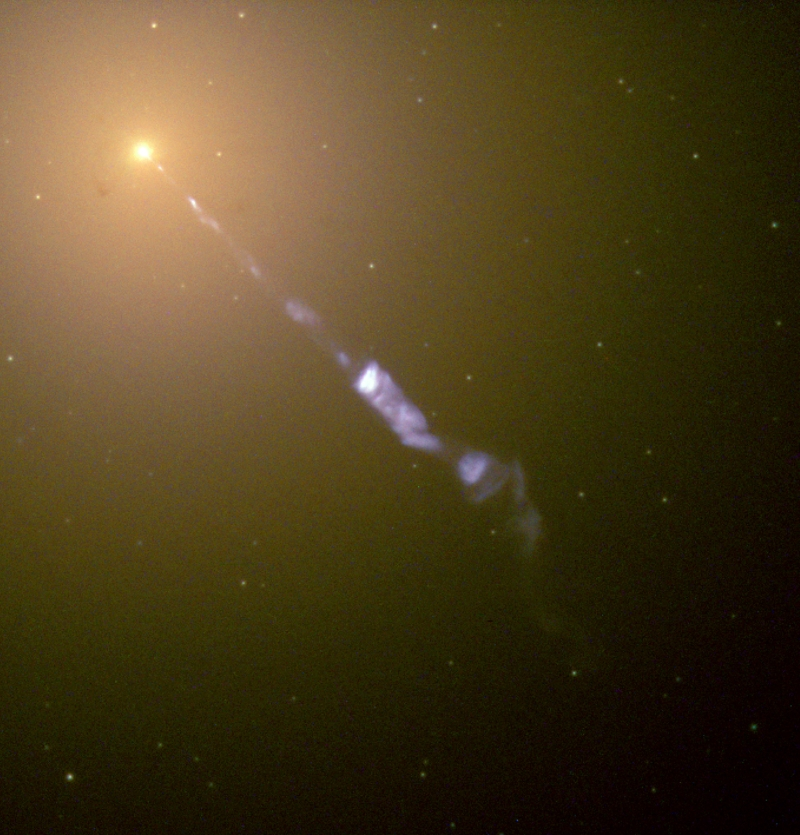
\includegraphics[width=0.5\textwidth]{images/M87_jet.jpg}
            \caption{M87, a giant elliptical galaxy with a jet. \emph{Image:
                NASA and The Hubble Heritage Team (STScI/AURA)}}
            \label{fig:m87}
        \end{figure}

        Electrons in jets can produce \emph{synchrotron radiation}, a form of
        radiation emitted by charged particles as they accelerate at
        relativistic speeds in a magnetic field \todo{citation needed}. This
        radiation is emitted in radio wavelengths, and so AGNs emitting this
        kind of radiation are called \emph{radio AGNs}. As radio AGNs are the
        focus of this thesis, from this point on ``AGN'' will refer only to
        radio AGNs.

        While we cannot observe the black holes of AGNs directly, we can observe
        the radio emissions from their jets. \todo{Keep motivating! Read those
        articles Julie suggested.}

        % \begin{figure}[!ht]
        %     \centering
        %     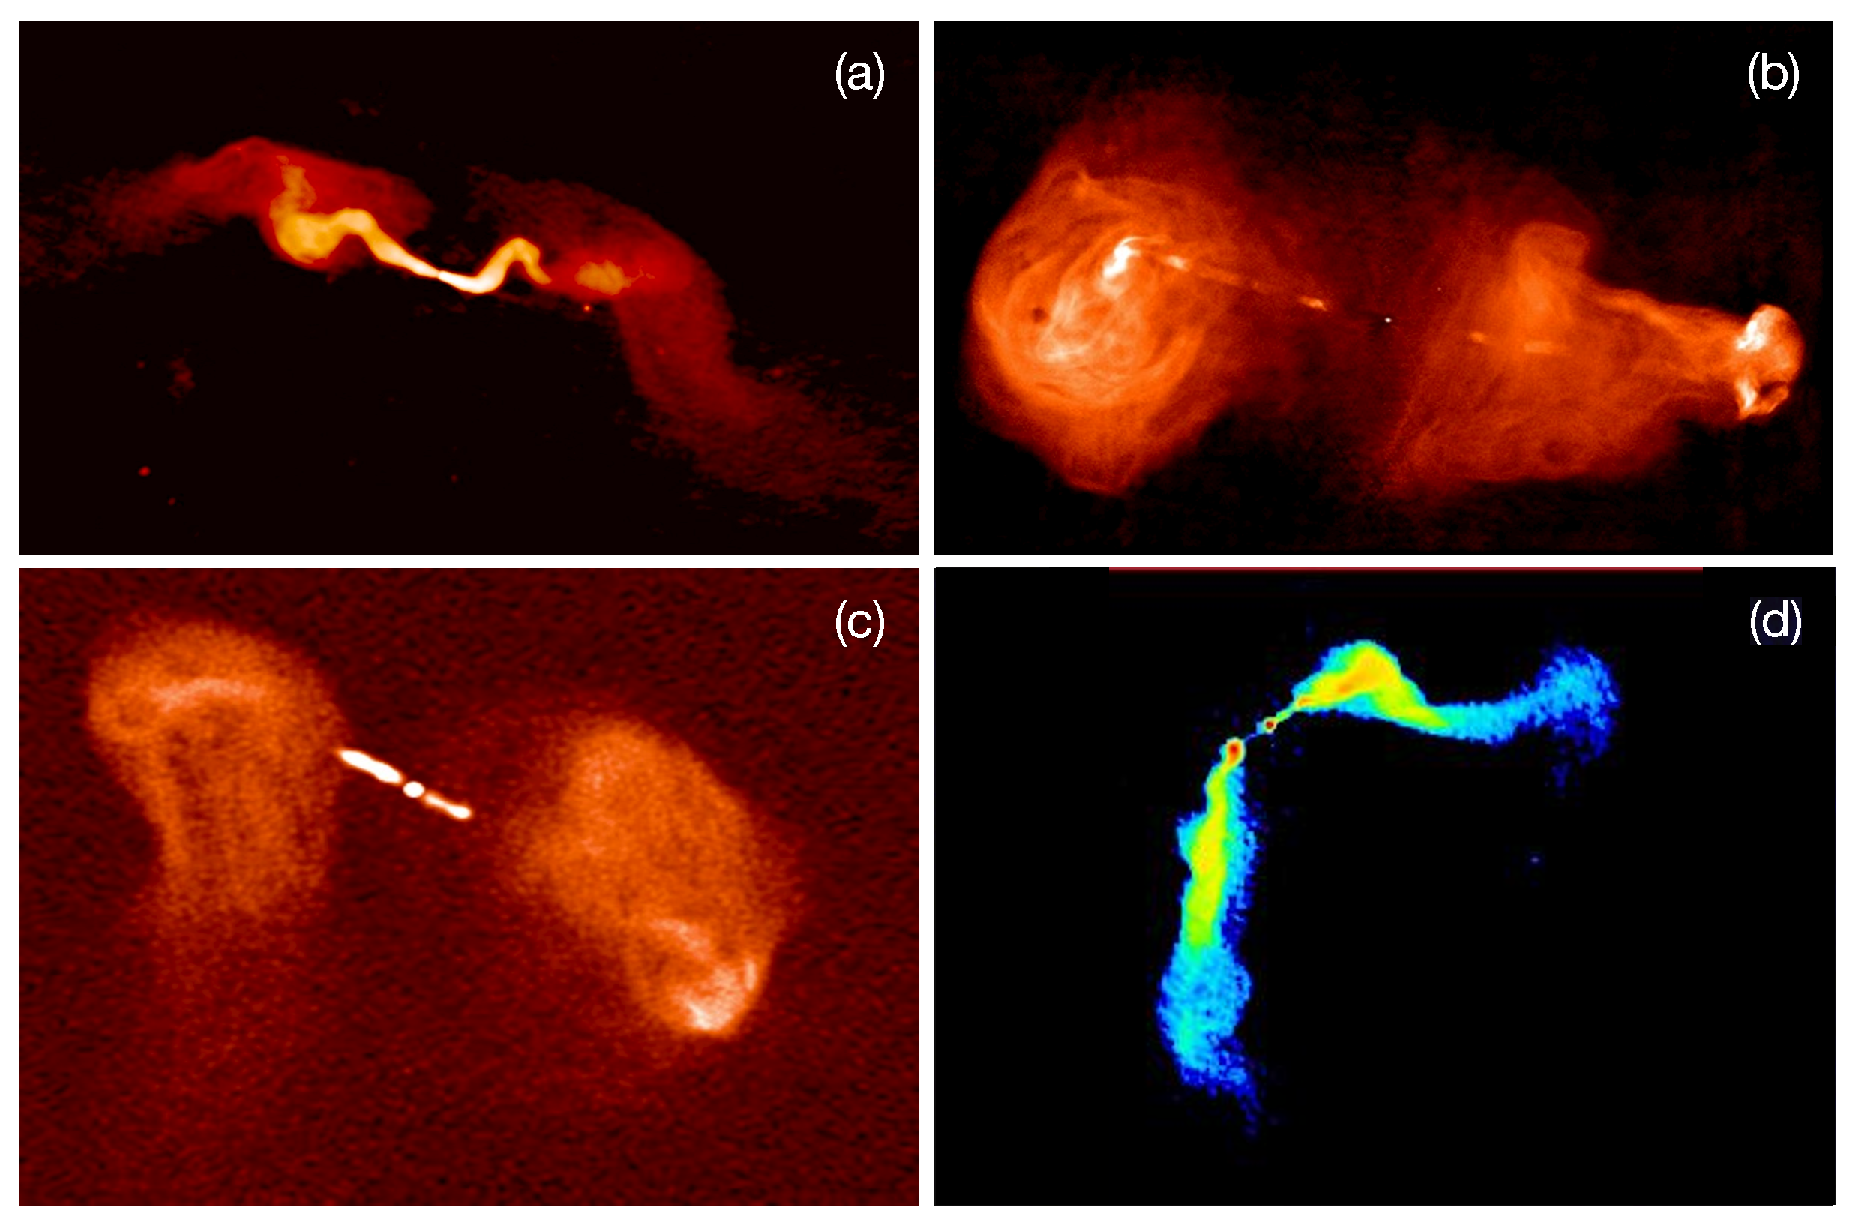
\includegraphics[width=0.8\textwidth]{images/rgz_fig1.eps}
        %     \caption{Different shaped radio AGNs. Figure reproduced from \citet{banfield15}.}
        %     \label{fig:radio-agns}
        % \end{figure}

    \section{Astronomical Observations}
    \label{sec:astronomical-observations}

        When observing the sky, we can think about the sky as a spherical
        surface surrounding the earth. All objects we see with telescopes are
        flat on the sky, and we only have limited tools to determine their
        distances and scales. In this section, I will describe the coordinate
        systems used to describe these objects, discuss some of the measurements
        we are able to make, and outline some of the challenges associated with
        astronomical observations.
        \todo{Fulfil these promises.}

        \subsection{Astronomical Coordinates}
        \label{sec:coordinates}

            Astronomy uses a coordinate system called the \emph{equatorial
            coordinate system} to describe the positions of objects on the sky.
            Each position on the sky is described by two numbers: the
            \emph{right ascension} (RA) and the \emph{declination} (dec).

            \begin{figure}[!ht]
                \centering
                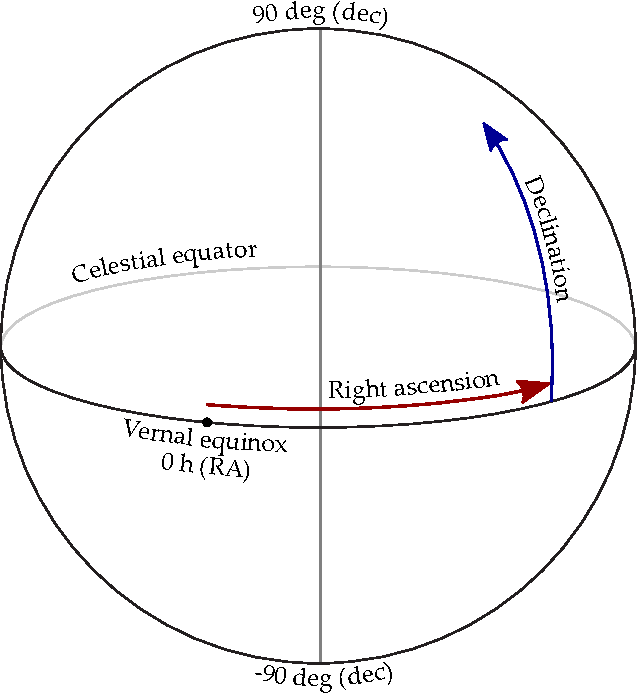
\includegraphics[width=0.5\textwidth]{images/ra-dec}
                \caption{The equatorial coordinate system.}
                \label{fig:equatorial-coordinates}
            \end{figure}

            The right ascension of an object is the angle eastward from the
            vernal equinox to the object along the celestial equator. It is
            measured in hours (h), minutes (min), and seconds (s). There are 60
            seconds in 1 minute, 60 minutes in 1 hour, and 1 hour is equal to 15
            degrees. Right ascension ranges between 0h and 24h, where both 0h
            and 24h are located at the vernal equinox. The declination of an
            object is the angle northward from the celestial equator to the
            object. It is measured in degrees (${}^\circ$), arcminutes ($'$),
            and arcseconds ($"$). Declination ranges between $-90^\circ$ and
            $90^\circ$, where $-90^\circ$ is the declination of the south
            celestial pole and $90^\circ$ is the declination of the north
            celestial pole. The right ascension and declination are shown in
            Figure \ref{fig:equatorial-coordinates}. It is important to note
            that while right ascension and declination are both measured in
            minutes and seconds, these are \emph{different} minutes and seconds.
            1 minute (right ascension) is equal to 15 arcminutes (declination).

            Objects are usually given a International Astronomical Union (IAU)
            name based on their coordinates. This name includes the catalogue
            that identified the object, the right ascension, and the
            declination. For example, ATLAS3 J002925.7-440256C is from the third
            release of the ATLAS catalogue, and is located at 00h 29m 25.7s
            $-44^\circ$ $02'$ $56"$.

            \todo{Write about epochs.}

            \todo{Figure out whether to talk about redshift.}

        % \subsection{Redshift}

        %     The \emph{redshift} $z$ of an object is a measure of the distance to
        %     that object based on the expansion of the universe. \todo{Finish
        %     this.}

        \subsection{Flux and Magnitude}

            The \emph{flux density} $f$ of an object is its energy output per
            unit time per unit area, and is measured in $\text{W m}^{-2}$. The
            flux density is given by
            \[
                f = \frac{1}{A}\frac{\text{d}E}{\text{d}t}
            \]
            We cannot usually measure the flux over all frequencies, so usually
            flux is observed over a specific frequency range $\Delta \nu$. The
            \emph{spectral flux density} is then the limit of this as the
            frequency range approaches zero, i.e.
            \[
                f_\nu = \frac{1}{A}\frac{\text{d}^2E}{\text{d}\nu\text{d}t}
            \]
            where $E$ is the energy received from the object, $A$ is the area of
            the object on the sky, and $\nu$ is the frequency. The spectral flux
            density is measured in janskys (Jy), an astronomical unit equal to
            $10^{-26} \text{ W m}^{-2} \text{ Hz}^{-1}$ \citep{francis08}.

            The \emph{apparent magitude} $m$ of an object is a logarithmic
            measure of its apparent brightness seen from Earth, relative to the
            star Vega \citep{francis08}. The difference between the magnitudes
            of two objects represents the ratio of their flux densities
            \begin{equation}
                \label{eq:magnitude-difference}
                m_2 - m_1 = -2.5 \log_{10} \left(\frac{f_2}{f_1}\right)
            \end{equation}
            and so the apparent magnitude is given by
            \begin{equation}
                \label{eq:apparent-magnitude}
                m = -2.5 \log_{10} \left(\frac{f}{f_{\text{Vega}}}\right)
            \end{equation}
            where $f$ is the flux density of the object and $f_{\text{Vega}}$ is
            the flux density of Vega, measured at the same frequency.

    \section{Radio Surveys}
    \label{sec:radio-surveys}

        \todo{Introduce surveys. Map a few of them.}

        \subsection{EMU: Evolutionary Map of the Universe}
        \label{sec:emu}

            The largest existing radio survey is currently the NRAO VLA Sky
            Survey (NVSS) \citep{condon98}, which covered the entire northern
            sky as far south as $-40^\circ$. However, NVSS is very shallow, only
            detecting objects brighter than $2.5$ mJy, and only resolving
            objects to $45''$. The deepest existing radio survey is of the SWIRE
            fields \citep{owen08}, which only covered around $0.1$ deg$^2$ of
            the sky, but to a depth of $0.015$ mJy with an angular resolution of
            $1.6''$. The Evolutionary Map of the Universe (EMU) is an upcoming
            deep radio survey that aims to provide both deep and wide coverage
            of the radio sky \citep{norris11}. EMU will be sensitive to objects
            to around $0.015$ mJy with an angular resolution of around $10''$,
            and cover the entire southern sky as far north as $30^\circ$. The
            survey is expected to find huge numbers of radio objects --- while
            ATLAS (Section \ref{sec:atlas}) has detected around 4000 radio
            objects, EMU is expected to find \emph{70 million}.

            Such large numbers of radio objects make analysis of the data
            considerably more difficult than analysis of existing surveys has
            been.

            \begin{itemize}
                \item We need to use machine learning to do things like cross-
                    identification, because the dataset is \emph{really big}
                \item EMU might find lots of new things
                \item ATLAS is a pilot survey for EMU
                \item Scientific purpose (Norris has a section on this)
            \end{itemize}

        \subsection{ATLAS: The Australia Telescope Large Area Survey}
        \label{sec:atlas}

            \begin{figure}[!ht]
              \centering
              \includegraphics[width=0.8\linewidth,]{images/CDFS_bitmap}
              \caption{ATLAS observations of CDFS. Reproduced from \citet{franzen15}.}.
              \label{fig:cdfs}
            \end{figure}

            The Australia Telescope Large Area Survey (ATLAS) is a deep
            \todo{define?} survey of two small areas of the sky in radio
            wavelengths, which aims to help understand the evolution of early
            galaxies \citep{norris06}. The Australia Telescope Compact Array was
            used to image the Chandra Deep Field South (CDFS) and the European
            Large Area ISO Survey - South 1 (ELAIS-S1) fields. These fields are
            areas of the sky with few nearby objects, meaning that observations
            in these fields are of very old, distant objects. These fields were
            chosen because they are the two fields imaged in the Spitzer Wide-
            area Infrared Extragalactic Survey (SWIRE, Section \ref{sec:swire})
            visible from the southern hemisphere. SWIRE produced high-resolution
            infrared images of its fields, allowing all objects detected in the
            ATLAS radio images to be compared with their infrared counterparts.

            \todo{Revise this section given that EMU has its own section above.}
            ATLAS is considered a pilot survey for the Evolutionary Map
            of the Universe (EMU), an upcoming radio survey of the entire
            southern sky at resolutions 45 times higher and angular resolutions
            4.5 times better than the benchmark NRAO VLA Sky Survey
            \citep{norris11b}. EMU will use the new Australian Square Kilometre
            Array Pathfinder (ASKAP) telescope to image the same radio
            frequencies as ATLAS at the same resolutions, so tools and methods
            developed to process and interpret ATLAS data are expected to work
            well on the data produced by EMU. While ATLAS covers a total area of
            6.4 deg$^2$, EMU will cover $75\%$ of the sky \citep{norris11b,
            norris16}. EMU is expected to detect around 70 million radio
            objects, compared to the 2.5 million currently known
            \citep{banfield15}.

            ATLAS provides both a catalogue of detected radio objects and a
            radio image of the CDFS and ELAIS-S1 fields. The CDFS image covers a
            total area of 3.7 deg$^2$ and the ELAIS-S1 image covers a total area
            of 2.7 deg$^2$. The CDFS image is shown in Figure \ref{fig:cdfs}.
            The catalogue is a list of all objects detected in the images with a
            peak or integrated flux more than 5 times the background noise
            levels. Each object has an associated survey identifier, an IAU
            name, a position on the sky of the peak flux, a peak flux density,
            an integrated flux density, an angular size, whether the object is
            extended or compact, and a spectral index, as well as uncertainties
            associated with each measurement \citep{franzen15}.

    \section{Infrared Surveys}
    \label{sec:infrared-surveys}

        \subsection{WISE: Wide-field Infrared Survey Explorer}
        \label{sec:wise}

            \begin{itemize}
                \item WISE is an all-sky survey
                \item Resolution, sensitivity
                \item Purpose
            \end{itemize}

        \subsection{SWIRE: Spitzer Wide-Area Infrared Extragalactic Survey}
        \label{sec:swire}

            The Spitzer Wide-Area Infrared Extragalactic Survey (SWIRE) is a survey of seven fields of the sky in infrared and wavelengths \citep{lonsdale03}. These fields --- ELAIS-S1, ELAIS-N1, ELAIS-N2, Lockman, CDFS, and Lonsdale --- are called the \emph{SWIRE fields}, totalling 63.2 $\deg^2$ in area. ELAIS-S1 and CDFS are in the southern sky; all other fields are in the northern sky.

            \begin{itemize}
                \item SWIRE is a narrow survey with high resolution
                \item SWIRE fields
                \item Resolution, sensitivity
                \item Purpose
                \item Compare to WISE
            \end{itemize}

    \section{Radio Cross-identification}
    \label{sec:radio-cross-identification}

        \subsection{Motivation}
        \label{sec:cross-identification-motivation}

        \subsection{Norris et al. Catalogue}
        \label{sec:norris}

        \subsection{Fan et al. Catalogue}
        \label{sec:fan}

    \section{Radio Galaxy Zoo}
    \label{sec:radio-galaxy-zoo}

        \todo{Rewrite this section.}

%     Radio Galaxy Zoo volunteers are first asked to select combinations of radio
%     objects that correspond to one radio source, and are then asked to select
%     the location of the corresponding host galaxy \citep{banfield15}. Each
%     radio subject is labelled by multiple volunteers. These labels are then
%     collated as follows. First, the most common combination of radio objects is
%     selected, and all labels that have a different combination are discarded.
%     This radio combination is called the consensus radio combination. Then, the
%     density of host location labels is estimated using Gaussian kernel density
%     estimation (KDE), and the highest density location is selected. This is
%     called the consensus host location. The consensus host location is then
%     matched to the nearest infrared object.

%     An alternative way to find the consensus host location is by using a
%     clustering algorithm such as $k$-means. Host locations are clustered and
%     the cluster containing the most locations is taken to represent the
%     consensus; the consensus location is then the mean of the cluster. This is
%     faster and more robust than using KDE, but requires $k$ to be known. $k$
%     can be estimated using an algorithm such as PG-means \citep{hamerly07} or by
%     choosing $k$ to minimise some information criterion \todo{cite:sklearn}.
%     The consensus labels for the data associated with this thesis were found in
%     this way, fitting a Gaussian mixture model to the host locations with the
%     number of Gaussians chosen to minimise the Bayesian information criterion.

%     Repeated volunteer labelling helps to reduce noise in the labels. This is
%     necessary as the volunteers are not experts, and may incorrectly label the
%     subject. The hope is that the majority of volunteers will correctly label
%     subjects, which seems to be the case for radio subjects where more than
%     75\% of volunteers agree \citep{banfield15}. The number of times a radio
%     subject is shown to different volunteers is called the redundancy. The
%     redundancy is 5 if the subject is a compact source, and 20 for all other
%     sources. These numbers were chosen based on the redundancy levels of the
%     original Galaxy Zoo project [Banfield, personal communication] \todo{Is
%     this how to cite personal communication? Alternatively, is this written
%     down somewhere?}. Since labels with radio combinations that disagree with
%     the consensus are discarded, the redundancy is usually lower in practice
%     when finding the host location. This can lead to very low redundancy input
%     to KDE, causing KDE to fail. This failure can usually be caught, but the
%     existing solution in this case is to take the mean of all host locations.
%     This is not the consensus host location in general. Another effect is that
%     since more complex sources have higher levels of disagreement in the radio
%     combination stage, more complex sources have more discarded volunteer
%     labels, and thus lower redundancy --- so more complex sources have more
%     noise in their labels.
